


\section{MOTIVATION}
Currently the main channel for job seekers are online job finding web sites, like indeed or  monster etc, that make the find finding process easily and decrease the recruitment time. But most such web sites only allow users to use key word to search the jobs, which makes job searching as tedious and blind task. For example, I used keyword ``Java'' to search jobs with location restriction like Mountain View, CA area on the job search engine indeed.com, the web site returned about 7,000 jobs, show in figure~\ref{fig:Indeed}. Because the number of results of job searching is huge but un-ranked, the job seeker has to review every job description. Since no one has enough time to read all the jobs in the searching result, so the actual quality of job searching service is low. This is a classic problem of information overload.


\begin{figure}[htbp]
  \centering
  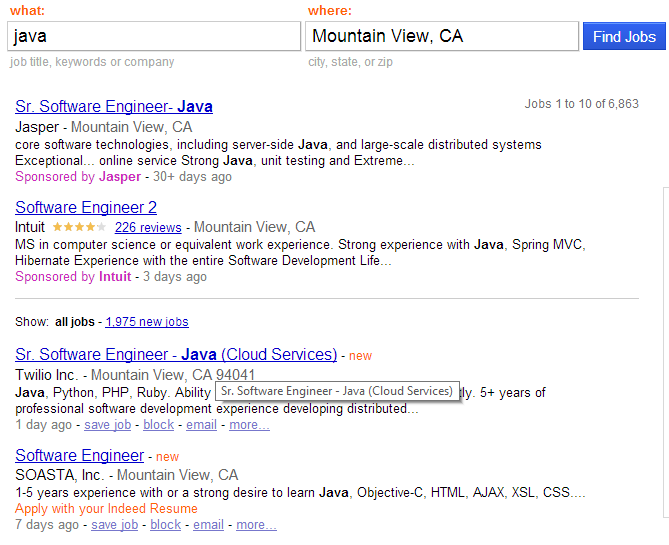
\includegraphics[scale=0.4]{images/indeed1.png}
  \caption{Search result of Indeed}
  \label{fig:Indeed}
\end{figure}

The reason for such result is because current job searching web site use the same information retrieval technology ``Inverted index'' \cite{zobel2006inverted} as in the common search engine, which just use keyword to map the docs that users want to search. Modern search engine all have ranking algorithms to sort the searching result, like page rank \cite{page1999pagerank}, so the top results always be the most related ones. But such algorithms for the job search engine is unavailable, because how to rank the job searching result is very personalized. A great job opening for one job seeker maybe means nothing to the other, the goodness of job for a specular job seeker is heavily depend on his personal background, like their education or professional experience etc.

Since the people's resumes contain the most important background information, we believe we can use the content of the resume to rank the job openings. My proposal is to create a web system which could use the resumes of job seekers to find the jobs that match their profiles best. The main idea is to build a job candidate model, which should be generated from resumes and job descriptions. I want to transfer the job searching task from key word searching to candidate model matching. The matching result should be sorted by the matching score, higher matching score means a better matching. Matching algorithm will not only help job seekers to find the appreciate job opening, but also offer priority to them.~\cite{gueutal2006brave}  The job with higher matching score means the job is more appropriate to the job seeker, and if he applies for the job, the chance of getting the interview will be higher as well. The figure~\ref{fig:Matching} will show how this approach works.


\begin{figure}[htbp]
  \centering
  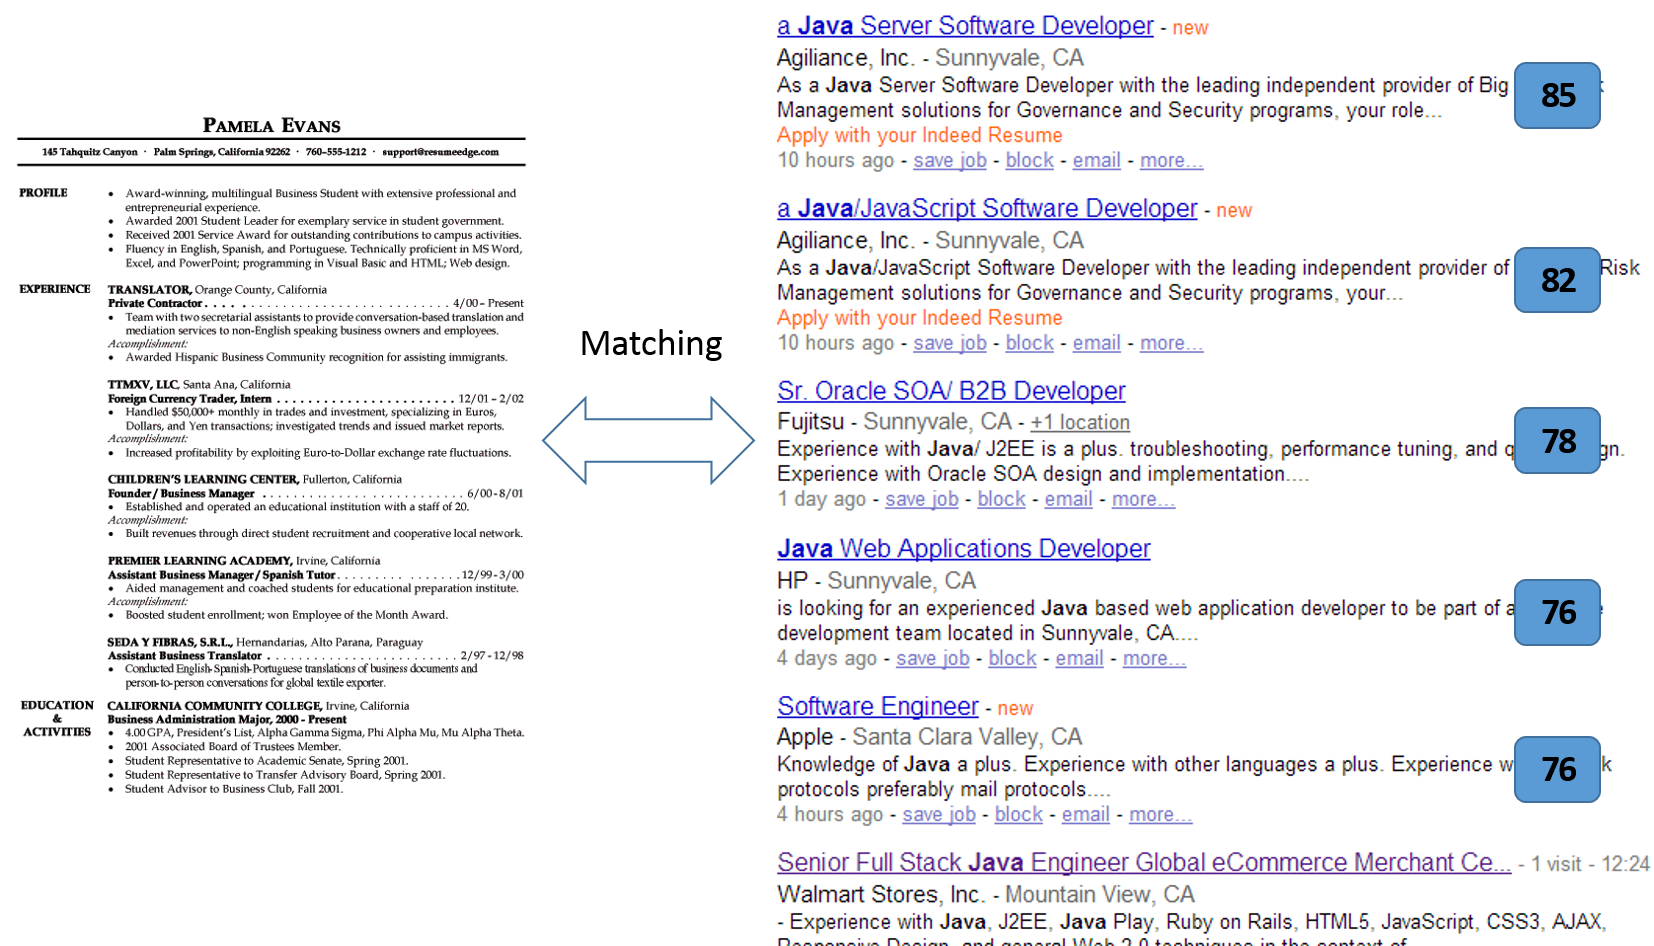
\includegraphics[scale=0.5]{images/matching.png}
  \caption{Matching the job opening with Resume}
  \label{fig:Matching}
\end{figure}

\section{PREVIOUS WORK}

Some scholars found that current Boolean search and filtering techniques cannot satisfy the complexity of candidate-job matching requirement.~\cite{malinowski2006matching} They hope the system could understand the job requirement, determine which requirements are mandatory and which are optional but preferable. So they move to use recommender systems techniques to address the problem of information overload

\subsection{Job Recommend System}

Job searching is not a new topic in information retrieval, it is been the focus of some commercial job finding web sites and research papers. Usually scholars call them Job Recommend System (JRS), because most of them used technology from other recommender systems. Recommend System could be classified into four categories~\cite{wei2007survey}: Collaborative Filtering, Content-based filtering, Knowledge-based and Hybrid approaches. Most of these technique had been applied in JRS. Zheng et al. ~\cite{siting2012job} and AlOtaibi et al.~\cite{al2012survey} summarized the categories of existing online recruiting platforms and listed the advantages and disadvantages of technical approaches in different JRSs.


\begin{enumerate}
    \item Content-based Recommendation (CBR) The principle of a content-based recommendation is to suggest items that have similar content information to the corresponding users, like Prospect \cite{singh2010prospect}.

    \item Collaborative Filtering Recommendation (CFR) Collaborative filtering recommendation, which finds  similar  users  who have  the same taste with the target user and recommends items based on what the similar users like, like CASPER~\cite{rafter2000personalised}.

    \item Knowledge-based Recommendation (KBR) In the knowledge-based recommendation, rules and patterns obtained from the functional knowledge of how a specific item  meets the requirement of a particular user, are used for recommending items, like  Proactive~\cite{lee2007fighting}.

\end{enumerate}

There are two main challenges in Content-Based Recommendation Systems, one is how to extract the information from the job opening and job seeker's resumes, the other is how to calculate similarity of them.

Lu et al~\cite{lu2013recommender}. use latent Semantic Analysis(LSA) to calculate similarities between jobs and candidates, but they selected only two factors ``interest'' and ``education''  to compare candidates.

\subsection{Information Extraction}
One important the problem of this system is how to extract the model from Job Description and Resume. The first step of model generating is information extraction. Both resume and job description are written in natural language, so we need to extract information from such un-structured or semi-structured data source.

Yu et al.~\cite{yu2005resume} use a cascaded information extraction (IE) framework to get the detailed information from the job
seeker��s resume. In the first stage, the Hidden Markov Modeling (HMM) model is used to segment the resume into consecutive blocks. Based on the result, a SVM model is used to obtain the detailed information in the certain block, such information include: name, address, education etc.

\subsection{Matching Algorithms}

Xing et al. ~\cite{yi2007matching} used a Structured Relevance Models (SRM) to  match resumes and jobs.

Ontology matching had been well studied by  Shvaiko and Euzenat in \cite{shvaiko2013ontology}

The Ontology technics had also been used in some JRSs. Proactive~\cite{lee2007fighting} use two kinds of ontology, one is job category and the other is company information. The system used ontology checker to classify the job information, store the domain knowledge and calculate the weight value in recommendations. In Ontology-based R��sum�� Parser (ORP) ~\cite{ccelik2013ontology},  Celik Duygua and Elci Atilla used ontology to assistant extract information from resumes. The system process the resume is following steps: convert the resume file to plain text, separate the text into  some segments, use Ontology Knowledge Base to find the concepts of the sentences, normalize all the terms, at last the system will classify the sentences to get the meaning.

Kumaran et al~\cite{kumaran2013towards} also used ontology to calculate the similarity between job criteria and candidates's resume in their system~\cite{kumaran2013towards}. The equation they use are:
$$ M\left ( i_1, i_2 \right ) = \frac{\sum_{k=1}^{n} Sim\left (p_{k}^{i1},  p_{k}^{i2} \right ) * W_{k}^{i2}}{\sum_{k=1}^{n} W_{k}^{i2}}  $$
The similarity function $Sim(p_1, p_2)$ is defined as follows:
$$ Sim(p1, p2) = \begin{Bmatrix}
1, & if~similarity~of~p1~and~p2 \geqslant t\\
0, & otherwise
\end{Bmatrix} $$

Fazel \cite{fazel2009semantic} used a hybrid approach to matching job seekers and job postings, which takes advantage of the benefits of both logic-based and ontology-based matching. In his paper the description logics (DL) is used to represent the candidate and job opening, and the ontology is used to organize the skills in a skill taxonomy. He gave an equation to calculate the matching degree:
$$ sim\left(P ,j \right) = \sum x_{ij} \times u(ds_i) $$

where, $x_{ji}$ is the Boolean variable indicating whether desire i is satisfied by applicant $A_{j}$ in the set of all qualified applications.

Liu and Dew~\cite{liu2004using} used RDF to represent and store the expertise of experts , and a RDF-based Expertise Matcher could retrieves the experts whose expertise include the required concept.

\section{METHODOLOGY}

The system will use Natural Language Processing, especially information extraction technique to parse the job description and resume, get information such as skill, specialties and background. This information will be used to build the model of job description and job seeker.  Ontology will be used to construct the knowledge base, which will include the taxonomy and rules, to support resume-job matching algorithm. Machine leaning algorithm will also be used to increase the accuracy of the matching algorithm by training with the existing data set.

The model of the candidate will include their specialties, working experience and education, all the information should be extracted from the resumes. The model also will be extracted from job description. When job seeker search the job, the system compares the candidate model from the resume to the models from the job descriptions.

In the initial phase I will only focus on the positions of IT job, because IT jobs have a special character,  skill set oriented, which means the person that the company want to hire must have some special skills and knowledge, like some programming languages, databases or software etc.

\subsection{System Architecture}

~\ref{fig:Pipeline} show the architecture of the whole system, which include such modules: 

\begin{enumerate}
    \item The web scrawler will search and download all new IT job opening web pages  from indeed.com everyday.
    \item Job parser will parse the job opening web page, extract the information and create the job model.
    \item Resume Parser is much like the Job parser, it will parser the resume and create the candidate model.
    \item All the job models will be stored in the Job Description database.
    \item When user make a query request, the ontology matcher will calculate the matching score of each job, return the jobs ranked by their scores.
\end{enumerate}

\begin{figure}[htbp]
  \centering
  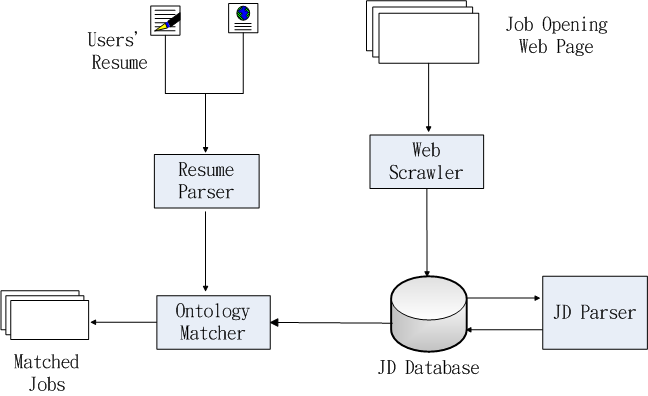
\includegraphics[scale=0.5]{images/arch.png}
  \caption{System Architecture}
  \label{fig:arch}
\end{figure}


\subsection{Information Extraction}
One important the problem of this system is how to extract the model from Job Description and Resume,
In Nature Language Processing, especially in Information Extraction, pipeline is a well adopted architecture~\cite{sarawagi2008information}. This system also use it to extract model of job opening and candidate's resume. The system will process the job opening in follow steps, which is show in ~\ref{fig:Pipeline}:

\begin{enumerate}
    \item HTML parser module will parse the job opening web pages that obtained from web scrawler module, get the HTML tag which has the mainly information of the job description.
    \item Segment module separate the job description into paragraphs according to HTML tag, then separate each paragraph into sentences
    \item The sentences will be tokenized, and sent to Classification module. This will determine the category of the sentence, and mark the category of the sentence.
    \item Preprocessing module will delete unreadable characters, normalize some spelling. 
    \item Annotation module will annotate the sentences with sematic and ontology labels. The sentences will be transferred to layered data structure.
    \item The layered sentences will be matched with predefined patterns. If any pattern could be matched, the ontology information will be stored in the job model.
    \item After every sentence has be processed in the pipeline, the job model will be stored into database.
\end{enumerate}


\begin{figure}[htbp]
  \centering
  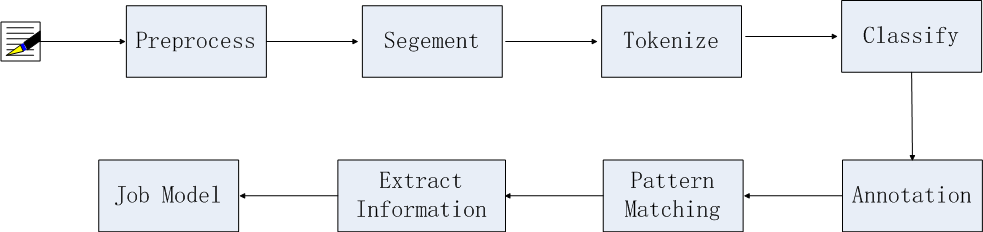
\includegraphics[scale=0.4]{images/pipeline.png}
  \caption{Job Description Process Pipeline}
  \label{fig:Pipeline}
\end{figure}

\subsection{Ontology Similarity}

But simple keyword of skill name matching is far from enough, because job description and resume are both written in human language, even the same things, they could be written in different ways. For example, below is part of the resume of a job seeker, and a part of a job description:

\begin{center}
\begin{tabular}{ | p{8cm} | p{7cm} | }
 \hline
   \textbf{Part of Resume}                 &   \textbf{Part of Job Description}   \\ \hline

    B.S. degree in computer science \newline
    5+ years Java, \newline
    2+ year   C++  \newline
    Some experience in Oracle database \newline
    Other experience like: \newline
    Hibernate, JBOSS, JUnit, Tomcat etc.
  &
  BS degree above   \newline
  4+ years Java  \newline
  Some experience of Python   \newline
    Mysql, MS-SQL   \newline
    Java web application Server   \newline
    OOA/OOD   \\
 \hline
\end{tabular}
\end{center}

If just looking at the text, we can find the resume has few common words with the job description.  But from the view of an experienced engineer, the candidate is pretty matching the job. Because relational databases Oracle and Mysql are very similar, OOA/OOD is the same meaning of many years of Java and C++ experience. Tomcat and JBOSS are two Java web applications.  But current key word searching technology won't give a good matching result in this very common situation. I believe ontology is a good solution to this system.
User��s personal preference should be considered as well. In the previous user survey, some factors will impact a lot on the user��s expectation of good jobs, such factors include: location, the reputation of the company, the salary etc. These factors will be treated with deferent weight in the job matching algorithm.


\section{SYSTEM FEATURES}

The system should include such features:

\begin{enumerate}
    \item User could import his resume in different format, like txt, doc and pdf.
    \item User could search jobs by his resume. The search result will be sorted by the matching scores.
    \item User could set their searching preference, like location, company type, reputation, salary level, etc.
    \item The system should learn user��s preference during the user��s searching process.
    \item The system should be able to change the parameters of the matching algorithm adaptively according to the record of user's preference
    \item The user could set multiple searching agents, each one of which is a composition of different preferences, like one for remote location with high salary, another for local company with low salary.
\end{enumerate}


\section{EVALUATION}

\subsection{Basic measures of the system}

In traditional information retrieval system, some measures are widely used~\cite{manning2008introduction}. These measures include:

\begin{enumerate}
    \item Precision ($P$) is the fraction of retrieved documents that are relevant .
       $$  Precision =  \frac{ \#(releveant~items~ retrieved)}{ \#(retrieved~items)}$$
    \item Recall ($R$) is the fraction of relevant documents that are retrieved.
       $$  Recall =  \frac{ \#(releveant~items~ retrieved)}{ \#(releveant~items)}$$
    \item $F measure$ ($F_1 score$) trades off precision versus recall.
       $$ F_1 = 2 \cdot \frac{ Precision \cdot Recall}{ Precision + Recall } $$
    \item Since the results are ranked, $ Normalized~Discounted~Cumulative~Gain ( NDCG )$ will be an important measure to evaluate the ranked retrieval results.
       $$ NDCG(Q,k) = \frac {1}{|Q|} \sum_{j=1}^{|Q|}{Z_{kj}} \sum_{m=1}^{k} \frac{2^{R(j,m)} - 1}{ \log_2(1+m)} $$
\end{enumerate}

\subsection{Evaluation Process}

Two methods will be used to evaluate the quality of the system:
1.	Pre-collected data: The user will be asked to use current job hunting web sites to find some jobs that he believes to be the best match. These jobs will be put into the system with some other random collected jobs.  When searching the jobs with the resume of the same user, we can get precision, recall and F measure of the system. The ranking position of the result is also very important, so NDCG is also a very important measure.

\subsection{User Experience}
2.	User experience:  The user will be asked to use both the system and current job finding web site. We can compare some factors to evaluate the system, such as:


\begin{enumerate}
    \item The time consumed to find satisfying jobs
    \item The quality of search results
    \item The user subjective experience with the both systems
\end{enumerate}


\section{TIME TABLE}
\begin{center}
\begin{tabular}{ |c|p{1cm}|p{1cm}|p{1cm}|p{1cm}|p{1cm}|p{1cm}| }
 \hline
  Content                 & May              & Jun             & Jul              & Aug             & Sep             & Oct  \\ \hline
  Literature Review       & \cellcolor{red}  & \cellcolor{red} &                  &                 &                 &      \\ \hline
  Data Collection         &                  & \cellcolor{red} & \cellcolor{red}  &                 &                 &      \\ \hline
  Requirement Analysis    &                  &                 & \cellcolor{red}  &                 &                 &      \\ \hline
  Implementation          &                  &                 &                  & \cellcolor{red} &                 &      \\ \hline
  Evaluation and Analysis &                  &                 &                  &                 & \cellcolor{red} &   \\ \hline
  Writing and Wrap Up     &                  &                 &                  &      & \cellcolor{red} & \cellcolor{red}     \\ \hline
  Defending               &                  &                 &                  &                 &     &  \cellcolor{red}    \\ \hline


 \hline
\end{tabular}
\end{center}

\section{CONCLUSION}

In this proposal I proposed a personalized job-resume matching system, which could help job seeker to find appropriate jobs more easily. In the system, job descriptions and resumes will be process by pipeline; and a finite automated tool will be used to extract the model of them. The job descriptions will be matched the user's resume, the result will be sorted by the ontology similarity. Since the most appreciate jobs will be returned in front of other jobs, the users of the system could get better result than current job finding web site.
